
\chapter{Curvature; radius of curvature}


%99. 
\section{Curvature}


The shape of a curve depends very largely upon the 
rate at which the direction of the tangent changes as the 
point of contact describes the curve. This rate of change 
of direction is called {\it curvature} and is denoted by $K$. 
We now proceed to find its analytical expression, first 
for the simple case of the circle, and then for curves in general.
\index{curvature}

%100. 
\section{Curvature of a circle}

Consider a circle of radius $R$. 

\begin{figure}[h!]
%\begin{tabular}{cc}
\begin{minipage}{\textwidth}
\begin{center}
%\vspace{1.0 cm}
%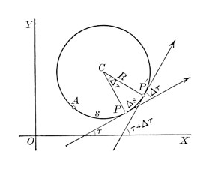
\includegraphics[height=3cm,width=6cm]{curvature-circle.eps}
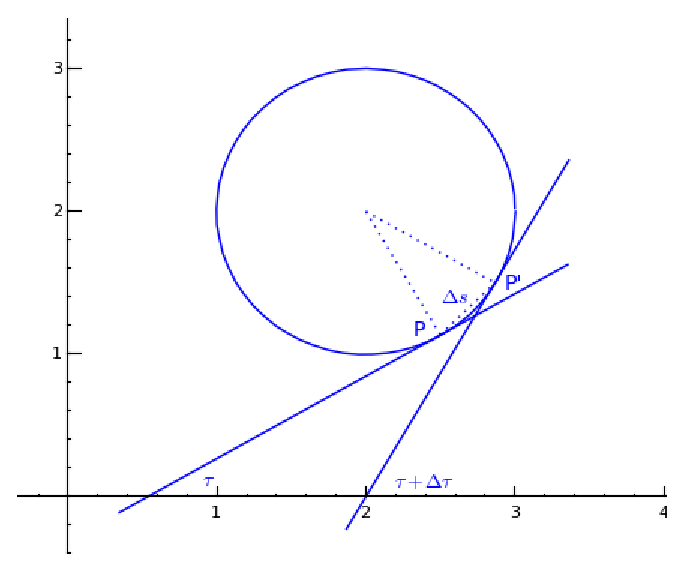
\includegraphics[height=5cm,width=6cm]{curvature-circle2.eps}
\end{center}
\end{minipage}
%\caption{Scan of Granville's graphic of the curvature of a circle.}
\caption{The curvature of a circle.}
\label{fig:curvature-circle}
\end{figure}
%sage: t = var("t")
%sage: f(t) = 2+cos(t)
%sage: g(t) = 2+sin(t)
%sage: tngt = lambda t, theta: ((g(theta)-2)*t+f(theta), -(f(theta)-2)*t+g(theta))
%sage: p1 = parametric_plot((f(t),g(t)), 0.0, 2*pi)
%sage: p2 = parametric_plot(tngt(t,-pi/6), -1.0, 2.0)
%sage: p3 = parametric_plot(tngt(t,-pi/3), -1.0, 2.5)
%sage: p4 = line([(2,2),(f(-pi/6),g(-pi/6))],linestyle=":")
%sage: p5 = line([(2,2),(f(-pi/3),g(-pi/3))],linestyle=":")
%sage: p6 = line([(f(-pi/3),g(-pi/3)),(f(-pi/6),g(-pi/6))],linestyle=":")
%sage: t1 = text("$\\tau$", (0.95,0.1))
%sage: t2 = text("$\\tau + \Delta \\tau$", (2.4,0.1))
%sage: t3 = text("$\Delta s$", (2.6,1.4))
%sage: t4 = text("P", (f(-pi/3)-0.13,g(-pi/3)+0.04))
%sage: t5 = text("P\'", (f(-pi/6)+0.13,g(-pi/6)))
%sage: show(p1+p2+p3+p4+p5+p6+t1+t2+t3+t4+t5)


Let 

\begin{center}
$\tau$ = angle that the tangent at P makes with the $x$-axis, 
\end{center}
and 

\begin{center}
$\tau + \Delta \tau$
= angle made by the tangent at a neighboring point P$'$.
\end{center}
Then we say $\Delta \tau$ = {\it total curvature} of arc PP$'$.
\index{total curvature}
If the point P with its tangent be supposed to move along 
the curve to P$'$, the total curvature ($= \Delta \tau$) 
would measure the total change in direction, or rotation, 
of the tangent; or, what is the same thing, the total 
change in direction of the arc itself. Denoting by $s$ 
the length of the arc of the curve measured from some 
fixed point (as A) to P, and by $\Delta s$ the length of 
the arc P P$'$, then the ratio
$\frac{\Delta \tau}{\Delta s}$
measures the average change in direction per unit 
length of arc\footnote{Thus, if 
$\Delta \tau = \frac{\pi}{6}$ radians (= $30^o$), and 
$\Delta s = 3$ centimeters, then 
$\frac{\Delta \tau}{\Delta s} = \frac{\pi}{18}$ radians 
per centimeter = $10^o$ per centimeter 
= average rate of change of direction.}. 
Since, from Figure \ref{fig:curvature-circle},
$  	\Delta s = R \cdot \Delta \tau$,
or $	\frac{\Delta \tau}{\Delta s} = \frac{1}{R}$,
it is evident that this ratio is constant everywhere 
on the circle. This ratio is, by definition, the 
curvature of the circle, and we have

\begin{equation}
%(38) 	
K = \frac{1}{R}.
\label{eqn:100-38}
\end{equation}
{\it The curvature of a circle equals the reciprocal of its radius.}

%101. 
\section{Curvature at a point}

Consider any curve. As in the last section,
$\Delta \tau$ = total curvature of the arc PP$'$,
and 
$\frac{\Delta \tau}{\Delta s}$ = 
average curvature of the arc PP$'$.

\begin{figure}[h!]
%\begin{tabular}{cc}
\begin{minipage}{\textwidth}
\begin{center}
%\vspace{1.0 cm}
%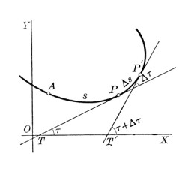
\includegraphics[height=3cm,width=6cm]{curvature-point.eps}
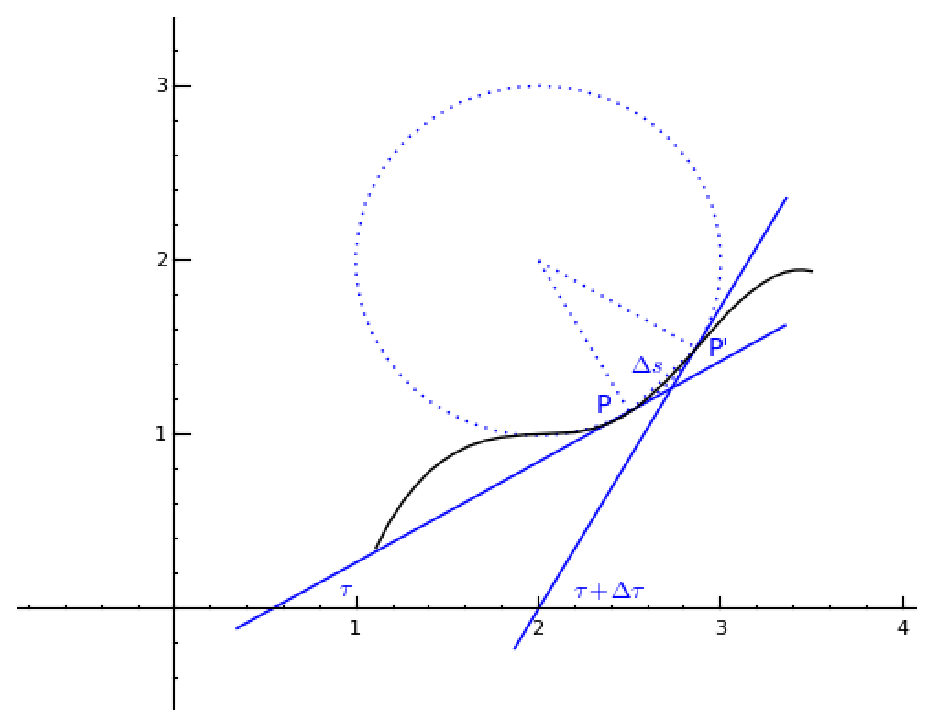
\includegraphics[height=6cm,width=7cm]{curvature-point2.eps}
\end{center}
\end{minipage}
%\caption{Scan of Granville's graphic of the curvature at a point.}
\caption{Geometry of the curvature at a point.}
\label{fig:curvature-point}
\end{figure}
%sage: t = var("t")
%sage: f(t) = 2+cos(t)
%sage: g(t) = 2+sin(t)
%sage: tngt = lambda t, theta: ((g(theta)-2)*t+f(theta), -(f(theta)-2)*t+g(theta))
%sage: p1 = parametric_plot((f(t),g(t)), 0.0, 2*pi, linestyle=":")
%sage: p2 = parametric_plot(tngt(t,-pi/6), -1.0, 2.0)
%sage: p3 = parametric_plot(tngt(t,-pi/3), -1.0, 2.5)
%sage: p4 = line([(2,2),(f(-pi/6),g(-pi/6))],linestyle=":")
%sage: p5 = line([(2,2),(f(-pi/3),g(-pi/3))],linestyle=":")
%sage: p6 = line([(f(-pi/3),g(-pi/3)),(f(-pi/6),g(-pi/6))],linestyle=":")
%sage: v = [(f(-pi/6),g(-pi/6)), (f(-pi/3),g(-pi/3)), (2,1)]
%sage: s = spline(v)
%sage: p7 = plot(s, 1.1, 3.5, rgbcolor=(0,0,0))
%sage: t1 = text("$\\tau$", (0.95,0.1))
%sage: t2 = text("$\\tau + \Delta \\tau$", (2.4,0.1))
%sage: t3 = text("$\Delta s$", (2.6,1.4))
%sage: t4 = text("P", (f(-pi/3)-0.13,g(-pi/3)+0.04))
%sage: t5 = text("P\'", (f(-pi/6)+0.13,g(-pi/6)))
%sage: show(p1+p2+p3+p4+p5+p6+p7+t1+t2+t3+t4+t5)


More important, however, than the notion of the average 
curvature of an arc is that of curvature at a point. 
This is obtained as follows. Imagine P to approach P 
along the curve; then the limiting value of the average 
curvature $\left( = \frac{\Delta \tau}{\Delta s} \right)$ 
as P$'$ approaches P along the curve is defined as the 
{\it curvature at P}, that is,
\index{curvature}

\begin{center}
Curvature at a point = 
$\lim_{\Delta s \to 0} \left( \frac{\Delta \tau}{\Delta s} \right) 
= \frac{d\tau}{ds}$.
\end{center}
Thefore,

\begin{equation}
%(39)
K = \frac{d\tau}{ds} = \ {\rm curvature}.
\label{eqn:101-39}
\end{equation}
Since the angle $\Delta \tau$ is measured in radians and 
the length of arc $\Delta s$ in units of length, 
it follows that the unit of curvature at a point is one 
radian per unit of length.

%102. 
\section{Formulas for curvature}
\label{sec:102}

It is evident that if, in the last section, instead 
of measuring the angles which the tangents made with 
the $x$-axis, we had denoted by $\tau$ and 
$\tau + \Delta \tau$ the angles made by the tangents with 
any arbitrarily fixed line, the different steps would 
in no wise have been changed, and consequently the results 
are entirely independent of the system of coordinates 
used. However, since the equations of the curves we 
shall consider are all given in either rectangular 
or polar coordinates, it is necessary to deduce 
formulas for $K$ in terms of both. We have
$\ \tan \tau 	= \frac{dy}{dx}$ by \S \ref{sec:32}, % 	§ 32, p. 31
or $\tau = \arctan \frac{dy}{dx}$.
Differentiating with respect to $x$, using XX in \S \ref{sec:33},

\[
%(A) 	
\frac{d\tau}{dx} 	
= \frac{ \frac{d^2 y}{dx^2} }{ 1 + \left( \frac{dy}{dx} \right)^2 }. 
\]
Also

\[
%(B) 	
\frac{ds}{dx} 	
= \left[ 1 + \left( \frac{dy}{dx} \right)^2 \right]^{\frac{1}{2}},
\]
by (\ref{eqn:24-90}). %p. 143 [§90]
Dividing one equation into the other %(A) by (B) 
gives

\[
\frac{ \frac{d\tau}{dx} }{ \frac{ds}{dx} } 	
= \frac{ \frac{d^2 y}{dx^2} }{ \left[ 1 
+ \left( \frac{dy}{dx} \right)^2 \right]^{\frac{3}{2}} }.
\]
But 	

\[
\frac{ \frac{d\tau}{dx} }{ \frac{ds}{dx} } 	
= \frac{d\tau}{ds} = K. 
\]
Hence

\begin{equation}
%(40) 	
K 	
= \frac{ \frac{d^2 y}{dx^2} }{ \left[ 1 
+ \left( \frac{dy}{dx} \right)^2 \right]^{\frac{3}{2}} }.
\label{eqn:102-40}
\end{equation}
If the equation of the curve be given in polar 
coordinates, $K$ may be found as follows:
From (\ref{eqn:B-67}), %p. 84 [§67],

\[
\tau 	= \theta + \psi. 
\]
Differentiating,

\[
%(C) 	
\frac{d\tau}{d\theta} 	
= 1 + \frac{d\psi}{d\theta}.
\]
But 	

\[
\tan \psi 	
= \frac{\rho}{\frac{d\rho}{d\theta}},
\]
from (\ref{eqn:A-67}). %p. 84 [§67]
Therefore, 

\[
\psi 	= \arctan \frac{\rho}{ \frac{d\rho}{d\theta} }.
\]
Differentiating with respect to $\theta$ using XX in \S \ref{sec:33}
and reducing,

\[
%(D) 	
\frac{d\psi}{d\theta} 	
= \frac{ \left( \frac{d\rho}{d\theta} \right)^2 
- \rho \frac{d^2 \rho}{d\theta^2} }{ \rho^2 
+ \left( \frac{d\rho}{d\theta} \right)^2 }.
\]
Substituting, %(D) in (C), 
we get

\[
%(E) 	
\frac{d\tau}{d\theta} 	
= \frac{\rho^2 - \rho \frac{d^2 \rho}{d\theta^2} 
+ 2 \left( \frac{d\rho}{d\theta} \right)^2}{\rho^2 
+ \left( \frac{d\rho}{d\theta} \right)^2}. 
\]
Also

\[
%(F) 	
\frac{ds}{d\theta} 	
= \left[ \rho^2 \left( \frac{d\rho}{d\theta} 
\right)^2 \right]^{\frac{1}{2}},
\]
by (\ref{eqn:30-91}). %, p. 136 [§91]
Dividing %(E) by (F) 
gives

\[
\frac{ \frac{d\tau}{d\theta} }{ \frac{ds}{d\theta} } 	
= \frac{ \rho^2 - \rho \frac{d^2 \rho}{d\theta^2} 
+ 2 \left( \frac{d\rho}{d\theta} \right)^2 }{ \left[ \rho^2 
+ \left( \frac{d\rho}{d\theta} \right)^2 \right]^{\frac{3}{2}} }.
\]
But 	

\[
\frac{ \frac{d\tau}{d\theta} }{ \frac{ds}{d\theta} } 	
= \frac{d\tau}{ds} = K. 
\]
Hence

\begin{equation}
%(41) 	
K 	
= \frac{ \rho^2 - \rho \frac{d^2 \rho}{d\theta^2} 
+ 2 \left( \frac{d\rho}{d\theta} \right)^2 }{ \left[ \rho^2 
+ \left( \frac{d\rho}{d\theta} \right)^2 \right]^{\frac{3}{2}} }.
\label{eqn:41-102}
\end{equation}

\begin{example}
{\rm
Find the curvature of the parabola 
$y^2 = 4px$ at the upper end of the 
latus rectum.

The {\it latus rectum} of a conic 
section is the chord parallel to the directrix and passing 
through the single focus, or one of the two foci. For more
details, see for example
\url{http://en.wikipedia.org/wiki/Semi-latus_rectum}.
\index{latus rectum}

Solution. 	
$\frac{dy}{dx} = \frac{2p}{y}$; 
$\frac{d^2 y}{dx^2} = - \frac{2p}{y^2} \frac{dy}{dx} = - \frac{4p^2}{y^3}$.
Substituting in (\ref{eqn:102-40}), 	
$K 	= -\frac{40-p^2}{( y^2 + 4p^2 )^{\frac{3}{2}}}$,
giving the curvature at any point. 
At the upper end of the latus rectum $(p, 2p)$,

\[
K = -\frac{4p^2}{ (4p^2 + 4p^2)^{\frac{3}{2}} } 	
= - \frac{4p^2}{16 \sqrt{2} p^3} = - \frac{1}{4 \sqrt{2} p}.
\]

While in our work it is generally only the numerical value 
of $K$ that is of importance, yet we can give a geometric 
meaning to its sign. Throughout our work we have taken the 
positive sign of the radical 
$\sqrt{1 + \left( \frac{dy}{dx} \right)^2}$. 
Therefore $K$ will be positive or negative at the same time that 
$\frac{d^2 y}{dx^2}$ is, i.e., (by \S \ref{sec:85}), %§85, p. 125), 
according as the curve is concave upwards or concave downwards.

We shall solve this using \sage.

\vskip .1in

\begin{Verbatim}[fontsize=\small,fontfamily=courier,fontshape=tt,frame=single,label=\sage]

sage: x = var("x")
sage: p = var("p")
sage: y = sqrt(4*p*x)
sage: K = diff(y,x,2)/(1+diff(y,x)^2)^(3/2)
sage: K
-p^2/(2*(p/x + 1)^(3/2)*(p*x)^(3/2))

\end{Verbatim}
\vskip .1in

\noindent
Taking $x=p$ and simplifying gives the result above.
\vskip .1in

\begin{Verbatim}[fontsize=\small,fontfamily=courier,fontshape=tt,frame=single,label=\sage]

sage: K.variables()
(p, x)
sage: K(p,p)
-p^2/(4*sqrt(2)*(p^2)^(3/2))
sage: K(p,p).simplify_rational()
-1/(4*sqrt(2)*sqrt(p^2))

\end{Verbatim}
}
\end{example}

\begin{example}
{\rm
Find the curvature of the logarithmic spiral 
$\rho = e^{a\theta}$ at any point.

Solution. 
$\frac{d\rho}{d\theta} = a e^{a\theta} = a \rho$; 
$\frac{d^2 \rho}{d\theta^2} = a^2 e^{a\theta} = a^2 \rho$.

Substituting in (\ref{eqn:41-102}), 
$K = \frac{1}{\rho \sqrt{1 + a^2}}$.

In laying out the curves on a railroad it will not do, 
on account of the high speed of trains, to pass abruptly from 
a straight stretch of track to a circular curve. In order 
to make the change of direction gradual, engineers make 
use of transition curves to connect the straight part 
of a track with a circular curve. Arcs of cubical parabolas 
are generally employed as transition curves.

Now we do this in \sage:

\vskip .1in

\begin{Verbatim}[fontsize=\small,fontfamily=courier,fontshape=tt,frame=single,label=\sage]

sage: rho = var("rho")
sage: t = var("t")
sage: r = var("r")
sage: a = var("a")
sage: r = exp(a*t)
sage: K = (r^2-r*diff(r,t,2)+2*diff(r,t)^2)/(r^2+diff(r,t)^2)^(3/2)
sage: K
1/sqrt(a^2*e^(2*a*t) + e^(2*a*t))
sage: K.simplify_rational()
e^(-(a*t))/sqrt(a^2 + 1)

\end{Verbatim}
}
\end{example}

\begin{example}
{\rm
The transition curve on a railway track has the shape of 
an arc of the cubical parabola $y = \frac{1}{3}x^3$. 
At what rate is a car on this track changing its 
direction ($1$ mi. = unit of length) when it is passing 
through (a) the point $(3, 9)$? (b) the point 
$(2, \frac{8}{3})$? (c) the point $(1, \frac{1}{3})$?

Solution. $\frac{dy}{dx} = x^2$, $\frac{d^2 y}{dx^2} = 2x$.
Substituting in (\ref{eqn:102-40}), 	
$K = \frac{2x}{(1 + x^4)^{\frac{3}{2}}}$.
(a) At $(3, 9)$, 
$K = \frac{6}{(82)^{\frac{3}{2}}}$ radians per mile = $28'$ per mile.
(b) At $(2, \frac{8}{3})$,
$K = \frac{4}{(17)^{\frac{3}{2}}}$ radians per mile = $3^o 16'$ 
per mile. 
(c) At $(1, \frac{1}{3})$, 	
$K = \frac{2}{(2)^{\frac{3}{2}}} = \frac{1}{\sqrt{2}}$ 
radians per mile = $40^o 30'$ per mile. 
}
\end{example}

%103. 
\section{Radius of curvature}
\label{sec:103}

By analogy with the circle (see (\ref{eqn:100-38})), %p. 156), 
the radius of curvature of a curve at a point is defined as 
the reciprocal of the curvature of the curve at that 
point. Denoting the radius of curvature by $R$, 
we have\footnote{Hence the radius of curvature will 
have the same sign as the curvature, that is, $+$ or $-$, 
according as the curve is concave upwards or concave downwards.}

\[
R = \frac{1}{K}.
\]
Or, substituting the values of $x$ from 
(\ref{eqn:102-40}) and (\ref{eqn:41-102}),

\begin{equation}
%(42) 	
R = \frac{ \left[ 1 
+ \left( \frac{dy}{dx} \right)^2 \right]^{\frac{3}{2}} }{ 
\frac{d^2 y}{dx^2} }
\label{eqn:103-42}
\end{equation}
and\footnote{In \S \ref{sec:98}, %§ 98, p. 152, 
%(43) is derived from (42) 
the next equation is derived from the previous one 
by transforming from rectangular to polar coordinates.}

\begin{equation}
%(43) 	
R = \frac{ \left[ \rho^2 
+ \left( \frac{d\rho}{d\theta} \right)^2 \right]^{\frac{3}{2}} }{ 
\rho^2 - \rho \frac{d^2 \rho}{d\theta^2} 
+ 2 \left( \frac{d\rho}{d\theta} \right)^2 }.
\label{eqn:43-103}
\end{equation}

\begin{example}
{\rm
Find the radius of curvature at any point of the catenary 
$y = \frac{a}{2} (e^{\frac{x}{a}} + e^{-\frac{x}{a}})$.

Solution. 	
$\frac{dy}{dx} 	
= \frac{1}{2} (e^{\frac{x}{a}} - e^{-\frac{x}{a}})$; 
$\frac{d^2 y}{dx^2} = \frac{1}{2a} (e^{\frac{x}{a}} - e^{-\frac{x}{a}})$.
Substituting in (\ref{eqn:103-42}),

\[
\begin{array}{ll}
R 
&= \frac{\left[ 1 + \left( \frac{e^{\frac{x}{a}} 
- e^{-\frac{x}{a}}}{2} \right)^2 \right]^{\frac{3}{2}} }{\frac{ 
e^{\frac{x}{a}} - e^{-\frac{x}{a}} }{2a}} \\
&= \frac{\left( \frac{ e^{\frac{x}{a}} 
- e^{-\frac{x}{a}} }{2} \right)^3}{ \frac{ e^{\frac{x}{a}} 
- e^{-\frac{x}{a}} }{2a}} = \frac{a (e^{\frac{x}{a}} - e^{-\frac{x}{a}})^2}{4} \\
= \frac{y^2}{a}.
\end{array}
\]
If the equation of the curve is given in parametric form, 
find the first and second derivatives of $y$ with respect to 
$x$ from (\ref{eqn:A-97}) and (\ref{eqn:B-97}), %pp. 150, 151, 
namely:

\[
%(G) 	
\frac{dy}{dx} 	= \frac{ \frac{dy}{dt} }{ \frac{dx}{dt} }, 
\]
and

\[
%(H) 	
\frac{d^2 y}{dx^2} 	
= \frac{ \frac{dx}{dt} \frac{d^2 y}{dt^2} 
- \frac{dy}{dt} \frac{d^2 x}{dt^2} }{ \left( \frac{dx}{dt} \right)^3 },
\]
and then substitute\footnote{Substituting 
these last two equations %(G) and (H), and then 
in (\ref{eqn:103-42}) gives 
$R = \frac{ \left[ \left( \frac{dx}{dt} \right)^2 
+ \left( \frac{dy}{dt} \right)^2 \right]^{3/2} }{ 
\frac{dx}{dt} \frac{d^2 y}{dt^2} 
- \frac{dy}{dt} \frac{d^2 x}{dt^2}}$.} 
the results in (\ref{eqn:103-42}).
}
\end{example}

\begin{example}
\label{ex:103-2}
{\rm
Find the radius of curvature of the cycloid
  	$x = a(t -\sin\, t)$, $y = a(t -\cos\, t)$.

Solution. 
$\frac{dx}{dt} = a(1 - \cos\, t)$, 
$\frac{dy}{dt} = a \sin\, t$;
$\frac{d^2 x}{dt^2} = a \sin\, t$,
$\frac{d^2 y}{dt^2} = a \cos\, t$.
Substituting the previous example %in (G) and (H), 
and then in (\ref{eqn:103-42}), %p. 159, 
we get

$\frac{dy}{dx} = \frac{\sin t}{1 - \cos t}$, 
$\frac{d^2 y}{dx^2} 
= \frac{ a(1 - \cos t) a \cos t - a \sin t a \sin t }{ a^3 (1 - \cos t)^3 } 
= \frac{1}{a(1 - \cos t)^2}$, and
$R = \frac{ \left[ 1 + \left( \frac{\sin t}{1 
- \cos t} \right)^2 \right]^{\frac{3}{2}} }{ -\frac{1}{a(1 
- \cos t)^2} } = -2a \sqrt{2 - 2 \cos t}$. 
}
\end{example}

%104. 
\section{Circle of curvature}
\label{sec:104}

Consider any point P on the curve $C$. The tangent drawn to 
the curve at P has the same slope as the curve itself 
at P (see \S \ref{sec:64}). %§ 64, p. 73). 
In an analogous manner we may construct for each point of the 
curve a circle whose curvature is the same as the curvature 
of the curve itself at that point. To do this, proceed as 
follows. Draw the normal to the curve at P on the concave 
side of the curve. 

\begin{figure}[h!]
%\begin{tabular}{cc}
\begin{minipage}{\textwidth}
\begin{center}
%\vspace{1.0 cm}
%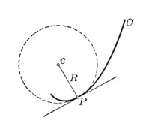
\includegraphics[height=3cm,width=3cm]{circle-curvature.eps}
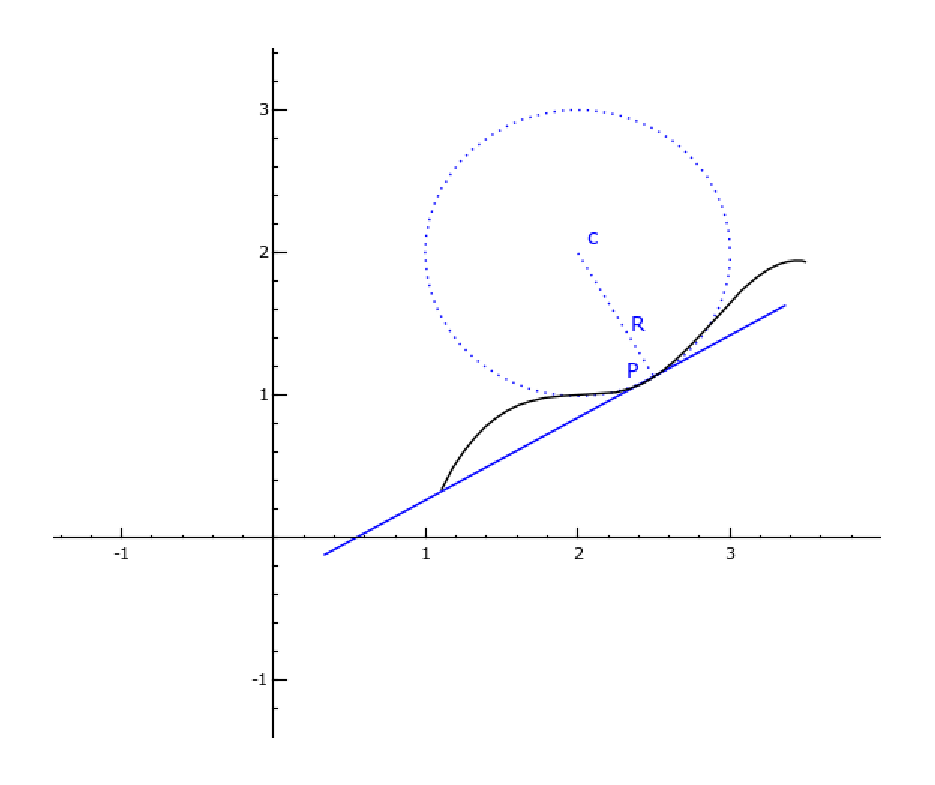
\includegraphics[height=6cm,width=7cm]{circle-curvature2.eps}
\end{center}
\end{minipage}
%\caption{Scan of Granville's graphic of the circle of curvature.}
\caption{The circle of curvature.}
\label{fig:circle-curvature}
\end{figure}
%sage: t = var("t")
%sage: f(t) = 2+cos(t)
%sage: g(t) = 2+sin(t)
%sage: tngt = lambda t, theta: ((g(theta)-2)*t+f(theta), -(f(theta)-2)*t+g(theta))
%sage: p1 = parametric_plot((f(t),g(t)), 0.0, 2*pi, linestyle=":")
%sage: p3 = parametric_plot(tngt(t,-pi/3), -1.0, 2.5)
%sage: p5 = line([(2,2),(f(-pi/3),g(-pi/3))],linestyle=":")
%sage: v = [(f(-pi/6),g(-pi/6)), (f(-pi/3),g(-pi/3)), (2,1)]
%sage: s = spline(v)
%sage: p7 = plot(s, 1.1, 3.5, rgbcolor=(0,0,0))
%sage: t1 = text("c", (2.1,2.1))
%sage: t2 = text("R", (2.4,1.5))
%sage: t4 = text("P", (f(-pi/3)-0.13,g(-pi/3)+0.04))
%sage: show(p1+p3+p5+p7+t1+t2+t4)


Lay off on this normal the distance 
PC = radius of curvature (= R) at P. With C as a center draw 
the circle passing through P. The curvature of this circle is then
$K = \frac{1}{R}$, which also equals the curvature of the curve 
itself at P. The circle so constructed is called the 
{\it circle of curvature} for the point P on the curve.
\index{circle of curvature}

In general, the circle of curvature of a curve at a point 
will cross the curve at that point. This is illustrated in the 
Figure \ref{fig:circle-curvature}.

Just as the tangent at P shows the direction of the curve at P, 
so the circle of curvature at P aids us very materially in 
forming a geometric concept of the curvature of the curve 
at P, the rate of change of direction of the curve and of 
the circle being the same at P.

%In a subsequent section (\S \ref{sec:116}) %§ 116) 
The circle of curvature can be 
defined as the limiting position of a secant circle, a 
definition analogous to that of the tangent given in 
\S \ref{sec:32}. %§ 32, p. 31.


\begin{example}
{\rm
Find the radius of curvature at the point $(3, 4)$ on the 
equilateral hyperbola $xy = 12$, and draw the 
corresponding circle of curvature.

Solution. 
$\frac{dy}{dx} = -\frac{y}{x}$, 
$\frac{d^2 y}{dx^2} = \frac{2y}{x^2}$.
For $(3, 4)$, 	
$\frac{dy}{dx} = -\frac{4}{3}$, 
$\frac{d^2 y}{dx^2} = \frac{8}{9}$, so

\[
R 	
= \frac{ [1 + \frac{16}{9}]^{\frac{3}{2}} }{ \frac{8}{9} } 
= \frac{125}{24} = 25\frac{5}{24}.
\]
The circle of curvature crosses the curve at two points.

We solve for the circle of curvature using \sage.
First, we solve for the intersection of the normal
$y-4=(-1/m)(x-3)$, where $m=y'(3)=-4/3$, and the circle
of radius $R=125/24$ about $(3,4)$:

\vskip .1in

\begin{Verbatim}[fontsize=\scriptsize,fontfamily=courier,fontshape=tt,frame=single,label=\sage]

sage: x = var("x")
sage: y = 12/x
sage: K = diff(y,x,2)/(1+diff(y,x)^2)^(3/2)
sage: K
24/((144/x^4 + 1)^(3/2)*x^3)
sage: K(3)
24/125
sage: R = 1/K(3)
sage: m = diff(y,x)(3); m
-4/3
sage: xx = var("xx")
sage: yy = var("yy")
sage: solve((xx-3)^2+(-1/m)^2*(xx-3)^2==R^2, xx)
[xx == -7/6, xx == 43/6]

\end{Verbatim}

\vskip .1in
\noindent
This tells us that the normal line intersects the circle of radius $R$ centered
at $(3,4)$ in 2 points, one of which is at $(43/6, 57/8)$. This is the center
of the circle of curvature, so the equation is $(x-43/6)^2+(y-57/8)^2=R^2$.


\begin{figure}[h!]
%\begin{tabular}{cc}
\begin{minipage}{\textwidth}
\begin{center}
%\vspace{1.0 cm}
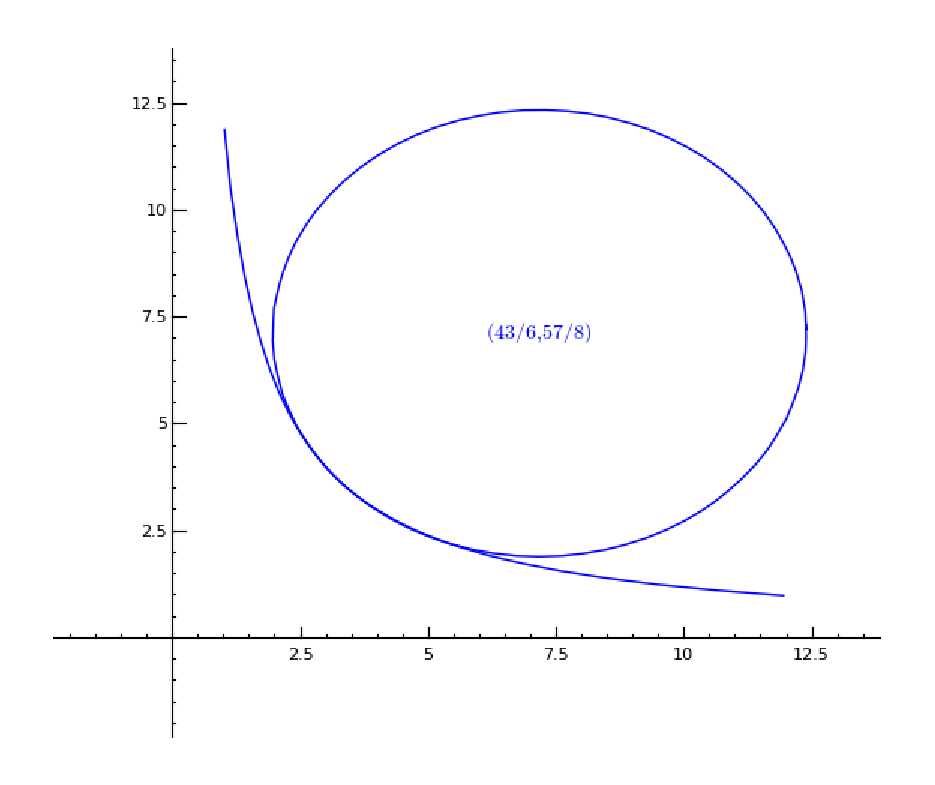
\includegraphics[height=5cm,width=6cm]{circle-curvature3.eps}
\end{center}
\end{minipage}
%\caption{Scan of Granville's graphic of the curvature of a circle.}
\caption{The circle of curvature of a hyperbola.}
\label{fig:circle-curvature3}
\end{figure}
%sage: p1 = plot(12/x,1,12)
%sage: p2 = parametric_plot([(125/24)*cos(t)+43/6, (125/24)*sin(t)+57/8], 0, 2*pi+0.1)
%sage: p3 = text("$(43/6,57/8)$", (43/6, 57/8))
%sage: show(p1+p2+p3)

}
\end{example}

\section{Exercises}

\begin{enumerate}
\item
%1
Find the radius of curvature for each of the following 
curves, at the point indicated; draw the curve and the 
corresponding circle of curvature:

\begin{itemize}
\item[(a)] 
$b^2x^2 + a^2y^2 = a^2b^2$, $(a,0)$. 	

Ans. 	$R = \frac{b^2}{a}$.

\item[(b)]
 $b^2y^2 + a^2y^2 = a^2b^2$, $(0,b)$.

Ans. $R = \frac{a^2}{b}$.

\item[(c)]
 $y = x^4 - 4x^3 - 18x^2$, $(0,0)$.

Ans. $R = \frac{1}{36}$.

\item[(d)]
 $16y^2 = 4x^4 - x^6$, $(2,0)$. 	  	

Ans. $R = 2$.

\item[(e)]
 $y = x^3$, $(x_1,y_1)$. 

Ans. $R = \frac{(1 + 9{x_1}^4)^{\frac{3}{2}}}{6x_1}$.

\item[(f)]
 $y^2 = x^3$, $(4,8)$.

Ans. $R = \frac{1}{3}(40)^{\frac{3}{2}}$.

\item[(g)]
 $y^2 = 8x$, $(\frac{9}{8}, 3)$. 

Ans. $R = \frac{125}{16}$.

\item[(h)]
 $\left( \frac{x}{a} \right)^2 
+ \left( \frac{y}{b} \right)^{\frac{2}{3}} = 1$, $(0, b)$. 	  	

Ans. $R = \frac{a^2}{3b}$.

\item[(i)]
 $x^2 = 4ay$, $(0,0)$. 

Ans. $R = 2a$.

\item[(j)]
 $(y - x^2)^2 = x^5$, $(0,0)$.

Ans. $R = \frac{1}{2}$.

\item[(k)]
 $b^2x^2 - a^2y^2 = a^2b^2$, $(x_1,y_1)$. 

Ans. $R = \frac{(b^4 {x_1}^2 + a^4 {y_1}^2)^{\frac{3}{2}}}{a^4 b^4}$.

\item[($\ell$ )]
 $e^x = \sin\, y$, $(x_1,y_1)$.

\item[(m)]
 $y = \sin\, x$, 
$\left( \frac{\pi}{2}, 1 \right)$. 

\item[(n)]
 $y = \cos\, x$, 
$\left( \frac{\pi}{4}, \sqrt{2} \right)$.

\item[(o)]
 $y = \log\, x$, $x = e$.

\item[(p)]
 $9y = x^3$, $x = 3$.

\item[(q)]
 $4y^2 = x^3$, $x = 4$.

\item[(r)]
 $x^2 - y^2 = a^2$, $y = 0$.

\item[(s)]
 $x^2 + 2y^2 = 9$, $(1, - 2)$.
\end{itemize}

\item
%2
 Determine the radius of curvature of the curve 
$a^2y = bx^2 + cx^2y$ at the origin.

Ans. $R = \frac{a^2}{2b}$.

\item
%3
Show that the radius of curvature of the witch 
$y^2 = \frac{a^2 (a - x)}{x}$ at the vertex is $\frac{a}{2}$.

\item
%4
Find the radius of curvature of the curve 
$y = \log\sec\, x$ at the point $(x_1,y_1)$.

Ans. $R = \sec\, x_1$.

\item
%5
Find $K$ at any point on the parabola 
$x^{\frac{1}{2}} + y^{\frac{1}{2}} = a^{\frac{1}{2}}$. 

Ans. $K = \frac{ a^{\frac{1}{2}} }{ 2(x + y)^{\frac{3}{2}} }$.

\item
%6
Find $R$ at any point on the hypocycloid 
$x^{\frac{2}{3}} + y^{\frac{2}{3}} = a^{\frac{2}{3}}$. 

Ans. $R = 3 (axy)^{\frac{1}{3}}$.

\item
%7
Find $R$ at any point on the cycloid 
$x = r \operatorname{arcvers} \frac{y}{r} - \sqrt{2ry - y^2}$. 

Ans. $R = 2 \sqrt{2ry}$.

\end{enumerate}

Find the radius of curvature of the following curves at any point:

\begin{enumerate}
\addtocounter{enumi}{7}

\item
%8
The circle $\rho = a\sin \theta$.

Ans. 
$R = \frac{a}{2}$.

\item
%9
The spiral of Archimedes $\rho = a\theta$.

Ans. $R = \frac{ (\rho^2 = a^2)^{\frac{3}{2}} }{ \rho^2 + 2a^2 }$.

\item
%10
The cardioid $\rho = a(1 − \cos\theta)$. 

$R = \frac{2}{3} \sqrt{2a\rho}$.

\item
%11
The lemniscate $\rho^2 = a^2\cos\, 2\theta$.

$R = \frac{a^2}{3\rho}$.

\item
%12
The parabola 
$\rho = a \sec^2 \frac{\theta}{2}$. 

Ans. $R = 2 a \sec^3 \frac{\theta}{2}$.

\item
%13
The curve $\rho = a sin^3 \frac{\theta}{3}$.

\item
%14
The trisectrix $\rho  = 2a\cos\theta - a$. 

Ans. $R = \frac{ a(5 - 4 \cos \theta)^{\frac{3}{2}} }{ 9 - 6 \cos \theta }$.

\item
%15
The equilateral hyperbola $\rho^2\cos\, 2\theta = a^2$. 

Ans. $R = \frac{\rho^3}{a^2}$.

\item
%16
The conic 
$\rho = \frac{a(1 - e^2)}{1 - e \cos \theta}$. 	

Ans. 
$R = \frac{a(1 - e^2)(1 - 2e \cos \theta + e^2)^{\frac{3}{2}}}{(1 
- e \cos \theta)^3}$.

\item
%17
The curve 	

\[
\begin{cases}
x = 3 t^2, \\ 
y = 3 t - t^3,
\end{cases}
\]
$t = 1$.

Ans. $R = 6$.


In \sage:

\vskip .1in

\begin{Verbatim}[fontsize=\scriptsize,fontfamily=courier,fontshape=tt,frame=single,label=\sage]

sage: x = 3*t^2
sage: y = 3*t-t^3
sage: R = (x.diff(t)^2+y.diff(t)^2)^(3/2)/(x.diff(t)*y.diff(t,2)-y.diff(t)*x.diff(t,2))
sage: R(1)
-6

\end{Verbatim}
\vskip .1in

\noindent

\item
%18
The hypocycloid 	

\[
\begin{cases}
x = a \cos^3 t, \\ 
y = a \sin^3 t,
\end{cases}
\]
$t = t_1$.

Ans. $R = 3a\sin\, t_1\cos\, t_1$.

In \sage:

\vskip .1in

\begin{Verbatim}[fontsize=\scriptsize,fontfamily=courier,fontshape=tt,frame=single,label=\sage]
sage: x = cos(t)^3
sage: y = sin(t)^3
sage: R = (x.diff(t)^2+y.diff(t)^2)^(3/2)/(x.diff(t)*y.diff(t,2)-y.diff(t)*x.diff(t,2))
sage: R
(9*cos(t)^2*sin(t)^4 + 9*cos(t)^4*sin(t)^2)^(3/2)/(-3*cos(t)^2*sin(t)*(6*cos(t)^2*sin(t) - 3*sin(t)^3) - 3*cos(t)*sin(t)^2*(6*cos(t)*sin(t)^2 - 3*cos(t)^3))
sage: R.expand()
(9*cos(t)^2*sin(t)^4 + 9*cos(t)^4*sin(t)^2)^(3/2)/(-9*cos(t)^2*sin(t)^4 - 9*cos(t)^4*sin(t)^2)

\end{Verbatim}
\vskip .1in

\noindent
You can simplify this last result using $\sin^2+\cos^2=1$.

\item
%19
The curve 	

\[
\begin{cases}
x = a(\cos t + t \sin t), \\ 
y = a(\sin t - t \cos t),
\end{cases} 	
\]
$t = \frac{\pi}{2}$.

Ans. $R = \frac{\pi a}{2}$.

\item
%20
The curve 	

\[
\begin{cases}
x = a(m \cos t + \cos mt), \\ 
y = a(m \sin t - \sin mt),
\end{cases} 	
\]
$t = t_0$.

Ans. $R = \frac{4 ma}{m - 1} \sin \left( \frac{m + 1}{2} \right) t_0$.

\item
%21
Find the radius of curvature for each of the following curves 
at the point indicated; draw the curve and the corresponding 
circle of curvature:

\begin{tabular}{ll}
(a) $x = t^2$, $2y = t$; $t = 1$. &	
(e) $x = t$, $y = 6t - 1$; $t = 2$.\\
(b) $x = t^2$, $y = t^3$; $t = 1$. &	
(f) $x = 2e^t$, $y = e^{-t}$; $t = 0$.\\
(c) $x = \sin\, t$, $y = \cos\, 2t$; $t= \frac{\pi}{6}$. &
(g) $x = \sin\, t$, $y = 2 \cos t$; $t = \frac{\pi}{4}$.\\
(d) $x = 1 - t$, $y = t^3$; $t = 3$. &
(h) $x = t^3$, $y = t^2 + 2t$; $t = 1$.\\
\end{tabular}

\item
%22
An automobile race track has the form of the ellipse 
$x^2 + 16y^2 = 16$, the unit being one mile. At what rate 
is a car on this track changing its direction

\begin{itemize}
\item[(a)] 
when passing through one end of the major axis?

\item[(b)] 
when passing through one end of the minor axis?

\item[(c)] 
when two miles from the minor axis?

\item[(d)] 
when equidistant from the minor and major axes?
\end{itemize}

Ans. (a) $4$ radians per mile; (b) $\frac{1}{16}$ radian per mile.

\item
%23
On leaving her dock a steamship moves on an arc of the 
semi cubical parabola $4y^2 = x^3$. If the shore line coincides with 
the axis of $y$, and the unit of length is one mile, how fast 
is the ship changing its direction when one mile from the shore?

Ans. $\frac{24}{125}$ radians per mile.

\item
%24
A battleship $400$ ft. long has changed its direction $30^o$ 
while moving through a distance equal to its own length. What is 
the radius of the circle in which it is moving?

Ans. $764$ ft.

\item
%25
At what rate is a bicycle rider on a circular track of 
half a mile diameter changing his direction?

Ans. $4$ rad. per mile = $43'$ per rod.

\item
%26
The origin being directly above the starting point, an aeroplane 
follows approximately the spiral $\rho = \theta$, the unit of 
length being one mile. How rapidly is the aeroplane turning at 
the instant it has circled the starting point once?

\item
%27
A railway track has curves of approximately the form of 
arcs from the following curves. At what rate will an engine 
change its direction when passing through the points 
indicated ($1$ mi. = unit of length):

\begin{tabular}{ll}
(a) $y = x^3$, $(2,8)$? &	
(d) $y = e^x$, $x = 0$?\\
(b) $y = x^2$, $(3,9)$? &
(e) $y = \cos\, x$, $x = \frac{\pi}{4}$?\\
(c) $x^2 - y^2 = 8$, $(3,1)$? &
(f) $\rho\theta = 4$, $\theta = 1$?\\
\end{tabular}

\end{enumerate}
